\begin{table}[H]
    {\renewcommand{\arraystretch}{1.2}%
    \setlength{\tabcolsep}{0.3em}%
\begin{tabular}{bababab}
\toprule

\rowcolor{white} \null &
\textbf{Synthetic$_{\mathbf{\mathcal{F}}}$} & \textbf{Synthetic$_{\mathbf{\mathcal{\beta}}}$} &
\textbf{Mine$_{\mathbf{\mathcal{F}}}$} & \textbf{Mine$_{\mathbf{\mathcal{\beta}}}$} &
\textbf{Office$_{\mathbf{\mathcal{F}}}$} & \textbf{Office$_{\mathbf{\mathcal{\beta}}}$} \\
\midrule

\rowcolor{lightgray}
\textbf{Keypoint Count} &
    \num{105788} & \num{23203} &
    \num{440400} & \num{440400} &
    \num{34200} & \num{34200} \\
\textbf{Correspondences} &
    \num{28836} & \num{5221} &
    \num{23132} & \num{13846} &
    \num{4172} & \num{2859} \\
\rowcolor{lightgray}
\textbf{True Positives} &
    \num{14047} & \num{3186} &
    \num{7688} & \num{2003} &
    \num{2131} & \num{1223} \\
\textbf{False Positives} &
    \num{27884} & \num{6148} &
    \num{144506} & \num{137922} &
    \num{10734} & \num{10632} \\
\rowcolor{lightgray}
\textbf{False Negatives} &
    \num{14789} & \num{2035} &
    \num{15444} & \num{11843} &
    \num{2041} & \num{1636} \\
\textbf{Precision} &
    \num{0.335} & \num{0.341} &
    \num{0.051} & \num{0.014} &
    \num{0.166} & \num{0.103} \\
\rowcolor{lightgray}
\textbf{Recall} &
    \num{0.487} & \num{0.610} &
    \num{0.332} & \num{0.145} &
    \num{0.511} & \num{0.428} \\
\textbf{Youden's index} &
    \num{0.123} & \num{0.268} &
    \num{-0.015} & \num{-0.179} &
    \num{0.146} & \num{0.082} \\
\rowcolor{lightgray}
\textbf{Accuracy} &
    \num{0.595} & \num{0.647} &
    \num{0.636} & \num{0.660} &
    \num{0.620} & \num{0.635} \\
\bottomrule
\end{tabular}

    }
    \caption{Performance indicators for the default configuration of the SIFT algorithm on the different datasets.}
\end{table}

Default configuration of SURF lead to massive amounts of keypoints for both flexion and bearing angle images.
They are clearly not distinguished do not stick to salient regions.
The cause of this issues seems to be, that on every octave the detector just adds all findings.
This could be a regression in the implementation, especially given the vastly different finding in prior work on \glspl{bearing-angle-image}.

To still get a climpse of the performance only one octave is used for detection and these keypoints are analyzed.
\begin{figure}[H]
\begin{subfigure}[t]{0.25\linewidth}
    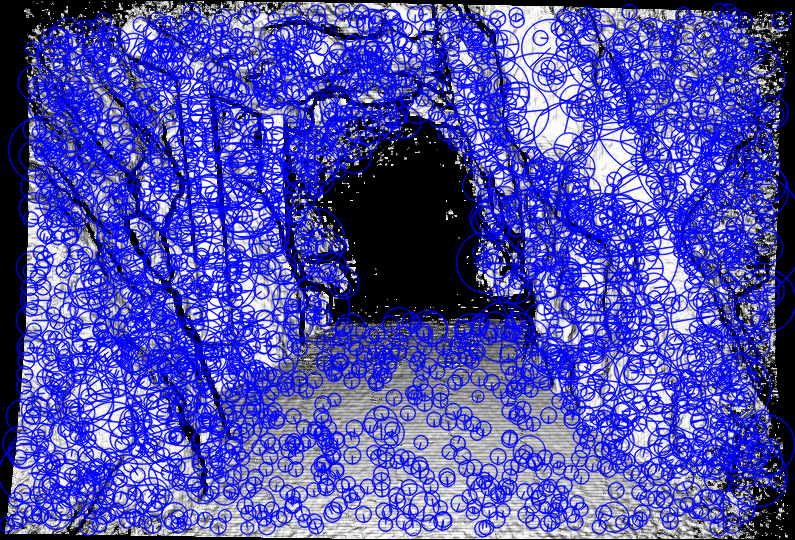
\includegraphics[width=\linewidth]{chapter06/results/SURF/flexion/default_kp0005.png}%
\end{subfigure}%
\begin{subfigure}[t]{0.25\linewidth}
    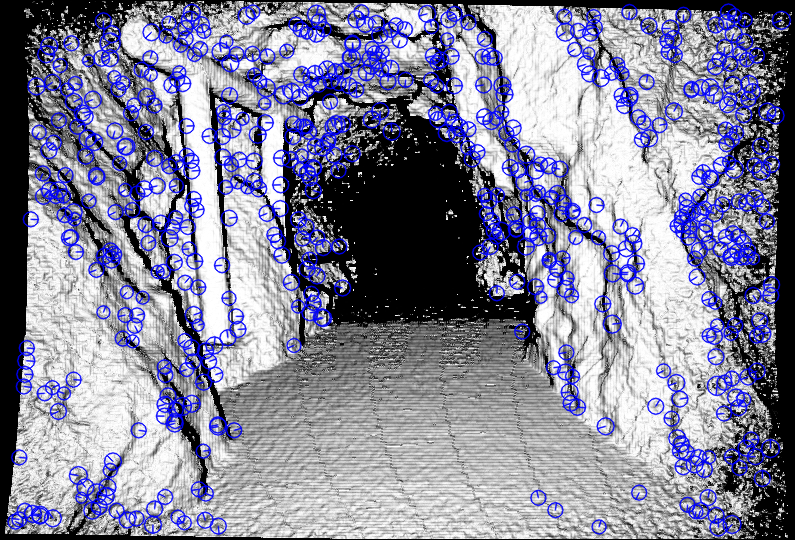
\includegraphics[width=\linewidth]{chapter06/results/SURF/flexion/oneoctave_kp0005.png}%
\end{subfigure}%
\begin{subfigure}[t]{0.25\linewidth}
    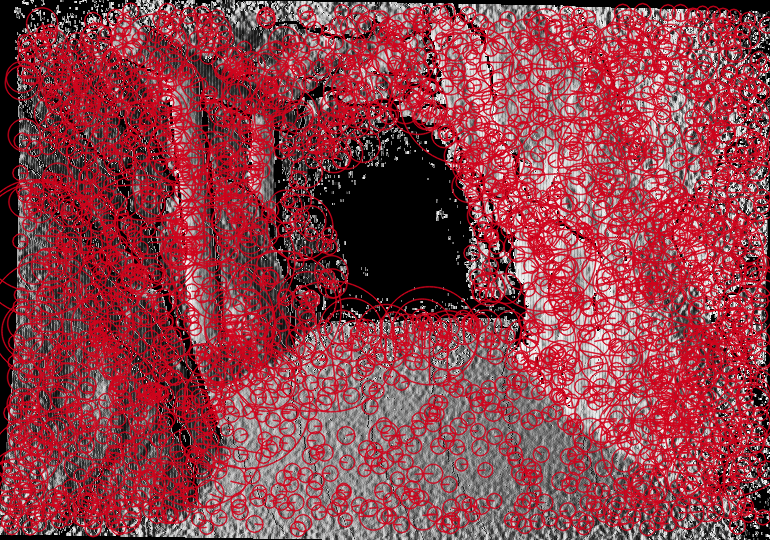
\includegraphics[width=\linewidth]{chapter06/results/SURF/bearing/default_kp0005.png}%
\end{subfigure}%
\begin{subfigure}[t]{0.25\linewidth}
    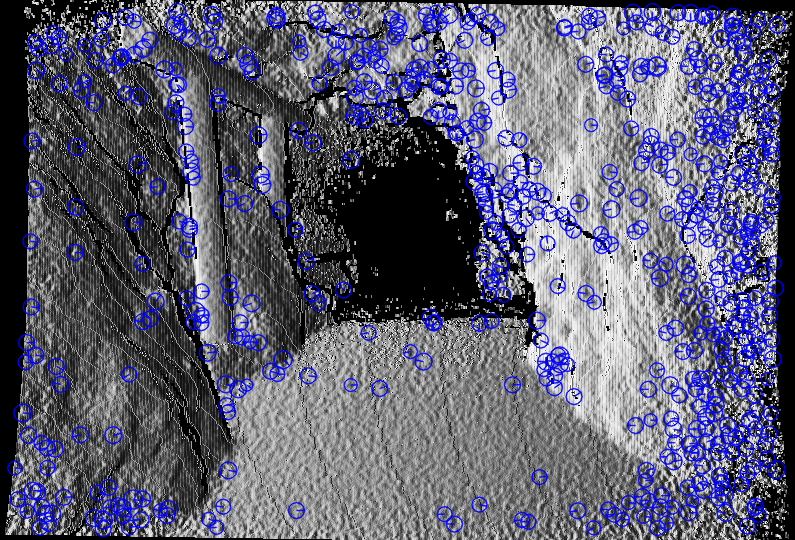
\includegraphics[width=\linewidth]{chapter06/results/SURF/bearing/oneoctave_kp0005.png}%
\end{subfigure}%
\caption{SURF configurations}
\end{figure}

\begin{figure}[H]
\begin{subfigure}[t]{0.45\linewidth}
    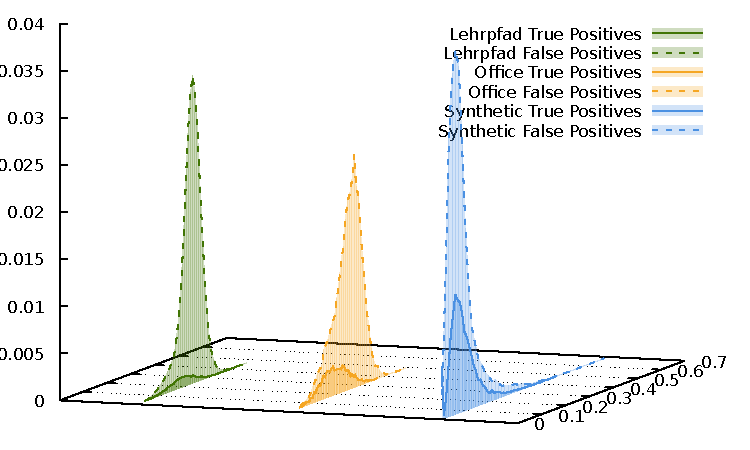
\includegraphics[width=\linewidth]{chapter06/results/SURF/flexion/descriptor_distances.pdf}%
    \caption{\gls{flexion-image} Descriptor Distances}
\end{subfigure}\quad
\begin{subfigure}[t]{0.45\linewidth}
    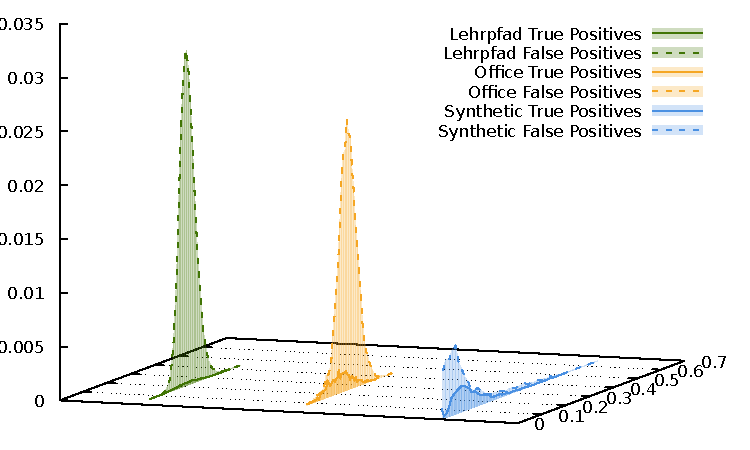
\includegraphics[width=\linewidth]{chapter06/results/SURF/bearing/descriptor_distances.pdf}%
    \caption{\gls{bearing-angle-image} Descriptors Distances}
\end{subfigure}
\end{figure}

\begin{figure}[H]
\begin{subfigure}[t]{0.45\linewidth}
    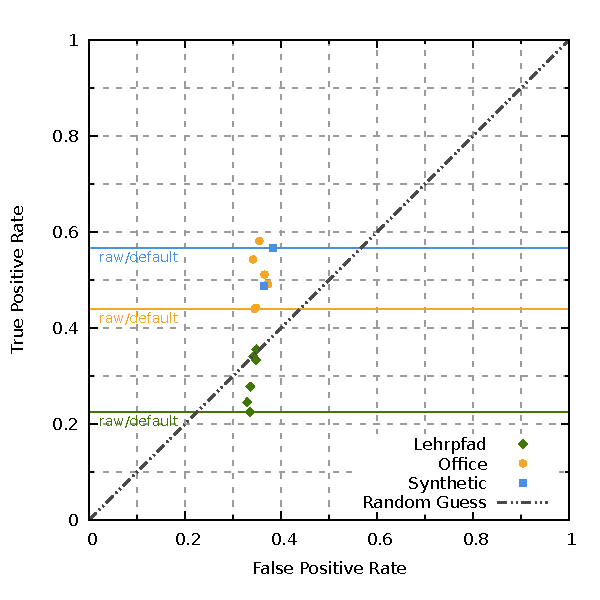
\includegraphics[width=\linewidth]{chapter06/results/SURF/flexion/roc.pdf}%
    \caption{Flexion Image ROC}
\end{subfigure}\quad
\begin{subfigure}[t]{0.45\linewidth}
    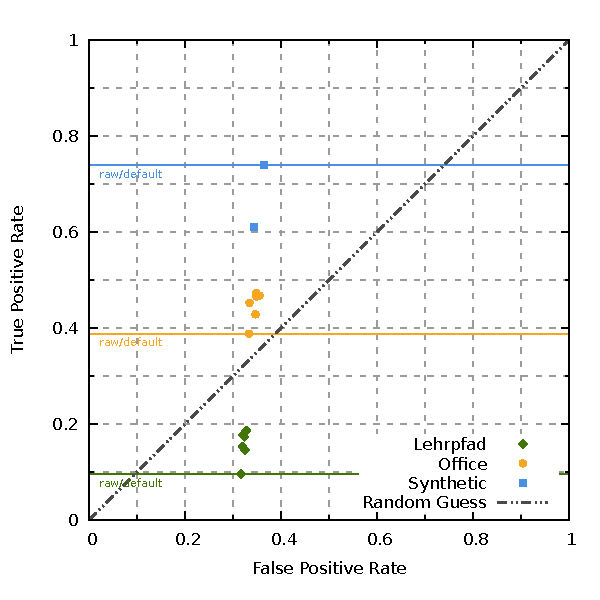
\includegraphics[width=\linewidth]{chapter06/results/SURF/bearing/roc.pdf}
    \caption{Bearing-Angle Image ROC}
\end{subfigure}
    \caption{Different Levels of Quality for SURF in the ROC plot.}
\end{figure}

